\section{\ddc{} Semantics}

The primitives of \ddc{} are deceptively simple.  Each captures a
simple concept, often familiar from type theory. However, in reality,
each primitive is multi-faceted. Each simultaneously describes a
collection of valid bit strings, two datatypes in the host language --
one for the data representation (Rep) itself and one for its parse
descriptor (PD) -- and a transformation from bit strings into data and
corresponding meta-data.

\reminder{
This paragraph is nice, but I don't think it belongs here.YHM 
What, then, are the semantics of a type? A number of factors went into
the design of \ddc{}, and they heavily influenced our choice for the
semantics of the calculus. First, it was necessary that the calculus
be simultaneously detailed enough to capture meaningful differences
between various data description languages (DDLs), and broad enough to
express the constructs found in these languages. Second, we sought to
explain to DDL users the process by which a bit stream is converted
into an in-memory representation. For the analyst, the data format
already existed, with a specific meaning. We sought to precisely
specify the transform so the analyst knows how that meaning is mapped
into the host language.  Finally, it was critical that \ddc{} include
error reporting and error handling mechanisms because errors are an
intrinsic characteristic of ad hoc data.
}
%All DDLs are set up to handle errors with varying degrees of flexibility.
%   (warn the reader that the current calculus is not necessarily
%   ultimately flexible in this regard, but open to extension).

We therefore choose to specify the semantics of \ddc{} with three
semantic functions, each precisely conveying a particular aspect of a
type's meaning. The function $\trans[\cdot,,]$ describes the {\it
  parsing semantics} of \ddc{}, defining a function in the lambda
calculus that parses bit strings to produce structured data and
meta-data. The functions $\itsem[\cdot]$ and $\itpdsem[\cdot]$
describe the {\it representation semantics} of \ddc{}, detailing the
in-memory representation of the data and meta-data -- the Rep and PD
types, respectively -- output by the parsing functions. The purpose
and relationship of the semantic functions is illustrated in
\figref{fig:correspond-graphic}. We note the structural correspondence
of Reps and PDs highlighted by the figure. 

\begin{table}
  \begin{center}
    \renewcommand{\arraystretch}{1.35}
    \begin{tabular}{l l}
      $\ddck[\ty,{\rctxt;\ctxt},\kind,\mcon]$ & {\it \ddc{}-type
        kinding}\\
      $\itsem[\ty] = \ity$ & {\it representation types of \ddc{} types}\\
      $\itpdsem[\ty] = \ity$ & {\it pd types of \ddc{} types}\\
      $\trans[\ty,\ctxt,\gk] = e$   & {\it \ddc{}-type semantics} \\
      $\kTrans[\gk,\ty] = \ity$     & {\it parser type} \\
      $\ptyc \rctxt = \ctxt$     & {\it context parser type}\\
      $\stsem[e,{\pctxt;\ctxt},\ity]$ & {\it \implang expression typing} \\
      $e \stepsto e'$ & {\it \implang expression evaluation}
    \end{tabular}
    \caption{Translations and Judgments}
    \label{tab:judg-list}
  \end{center}
\end{table}

In the remainder of this section, we formalize this three-fold
semantics of \ddc{} types.  For reference, we provide in
\tblref{tab:judg-list} a listing of all the functions and judgments
defined in this section and a brief description of each.  
\reminder{Should we define here $\rctxt,\ctxt,\pctxt$? --Kathleen}

\begin{figure}[tp]
  \centering
  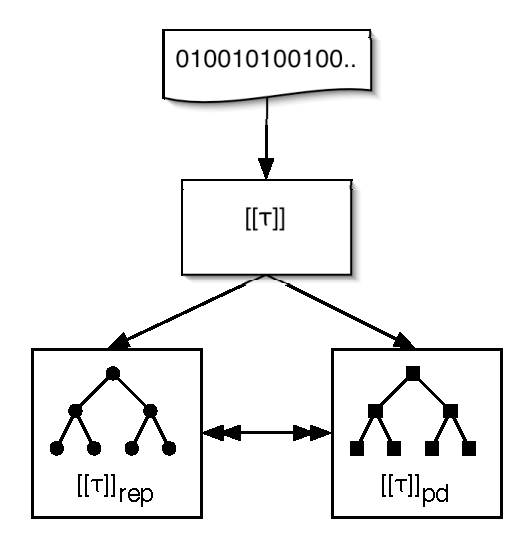
\includegraphics[height=2in,width=2in]{correspond}  
  \caption{Relationship between semantics functions}
  \label{fig:correspond-graphic}
\end{figure}

\subsection{Representation Semantics}
\label{sec:intty-sem}

As \implang{} Rep and PD types belong to the host language, we now
introduce those types.

\begin{bnf}
  \name{Base Types} \meta{a} \::= 
  \iboolty \| \iintty \| \iunitty \| 
  \invty \nlalt \iecty \| \ioffty \| \ibitsty
  \\
  \name{Types} \meta{\ity} \::= 
      \ibasety \| \iarrow \ity \ity \| \iprod \ity \ity \|
      \isum \ity \ity \nlalt
      \iseq \ity \| \forall \ityvar.\ity  \| \ityvar \|
      \imu \ityvar \ity   
\end{bnf}

\reminder{Should we fold this paragraph into the text below,
  introducing the types as they appear? --YHM} We highlight the
non-standard types of the language. The type $\invty$ is the singleton
type of the constant $\ierr$, most often injected into a sum when a
parse fails. Types $\iecty$ and $\ioffty$ are for error codes recorded
in the parse descriptors and bit-stream offsets, respectively.

The remaining types have their standard meaning: function types,
product types, sum types, sequence types $\iseqty \ty$; polymorphic
types $\forall \ityvar.\ity$ and type variables $\ityvar$; and
recursive types $\imu \ityvar \ity$.

\begin{figure}
\fbox{$\itsem[\ty] = \ity$}
\[
\begin{array}{lcl} 
\itsem[\ptrue] & = & \iunitty \\
\itsem[\pfalse] & = & \invty \\
\itsem[\pbase{e}] & = & \isum {\Irty(C)} \invty   \\
\itsem[\plam{\var}{\ity}{\ty}] & = & \itsem[\ty] \\
\itsem[\papp \ty e] & = & \itsem[\ty] \\
\itsem[\psig \var {\ty_1} {\ty_2}]  & = & \iprod {\itsem[\ty_1]} {\itsem[\ty_2]}    \\
\itsem[\psum {\ty_1} e {\ty_2}]     & = & \isum {\itsem[\ty_1]} {\itsem[\ty_2]} \\
\itsem[\pand {\ty_1} {\ty_2}]  & = & \iprod {\itsem[\ty_1]}{\itsem[\ty_2]}\\
\itsem[\pset x \ty e] & = & \isum {\itsem[\ty]}{\itsem[\ty]}\\
% field names: length, elts
\itsem[\pseq \ty {\ty_{\text{sep}}} {\pterm e {\ty_{\text{term}}}}] & = & 
    \iprod \iintty {(\iseq{\itsem[\ty]})}             \\
%% \itsem[\pcase e c {\ty_1} {\ty_2}]       & = & \isum {\itsem[\ty_1]} {\itsem[\ty_2]}\\
\itsem[\ptyvar] & = & \ptyvar \\
\itsem[\pmu \ptyvar \ty] & = & \imu{\ptyvar}{\itsem[\ty]} \\
\itsem[\pcompute e \ity]                 & = & \ity \\
\itsem[\pabsorb \ty]                     & = & \isum \iunitty \invty \\
\itsem[\pscan \ty] & = & \isum {\itsem[\ty]} \invty 
%% \pext{
%% \itsem[\ptransform e e \ty]              & = & \itsem[\ty]\\
%% }
\end{array}
\]
\caption{Representation Types}
\label{fig:rep-tys}
\end{figure}

In Figure~\ref{fig:rep-tys}, we present the in-memory representation
of each primitive of \ddc{}. We note that, as \ddc{} contains
dependent types while the \implang{} language is simply typed, an
essential feature of the translation is to detail how the dependency
is removed, which we now explain. For all basic types in which
expressions appear -- base, set, sequence and compute types, those
expressions are relevant only to parsing.  Hence, the translation
simply drops the expressions to remove the dependency. With these
expressions gone, variables become useless, and, hence, variable
bindings are dropped as well, as in product and set types. We raise
this approach to higher-order types by translating type abstraction
and application according to their underlying types~\footnote{Type
  abstractions do not really have a representation, as they cannot
  directly describe data. The value of defining the representation of
  type abstractions comes only from the fact that we determine the
  representation for applications from the underlying type
  (abstraction) being applied.}.

The \ddc{} type $\ptrue$ transforms no input and hences produces only
the $\iunitty$ value.  Correspondingly, $\pfalse$ transforms no input,
but uniformly fails, and hence produces the $\invty$ value. The
function $\Irty$ maps each base type to a representation for
successfully parsed data. As base type parsers can fail, this type is
summed with $\invty$ to produce the actual representation. Similarly,
set types produce sums, where a left branch indicates that the data
satisfied the contraint, and the right indicates that it did not.�In
the latter case, though, as the error is semantic rather than
syntactic, the parser can return the offending data rather than $\ierr$.

Intersection types produce a pair of values -- one for each sub-type
-- as the representations of the subtypes need not be identical nor
even compatible. Sequences produce an sequence together with its
length.  Recursive types generate recursive \implang{} data
structures. Note that the \implang{} type uses the same variable names
as the \ddc{} type, and so the type corresponding to the type variable
$\ptyvar$ is exactly $\ityvar$.

The output of a $\pcomputen$ is exactly the computed value, and,
therefore shares its type.  The output of $\pabsorbn$ is a sum
indicating whether parsing the underlying type succeeded or failed.
The type of $\pscann$ is similar, although instead returning an
element of the underlying type in case of success.

\begin{figure}
\fbox{$\itpdsem[\ty] = \ity$}
\[ 
\begin{array}{lcl} 
%% %% example: \ua.(int * a) + None
%% %%          pd = \ua.pd_hdr  * ((pd_hdr * ([int]_pd * [a]_pd)) + [None]_pd)
%% %%             = \ua.pd_hdr  * ((pd_hdr * ([int]_pd * a)) + [None]_pd)

\itpdsem[\ptrue] & = & \ipty \iunitty \\                                                  
\itpdsem[\pfalse] & = & \ipty \iunitty \\                                                  
\itpdsem[\pbase{e}] & = & \ipty \iunitty\\
\itpdsem[\plam \var \ity \ty] & = & \itpdsem[\ty] \\
\itpdsem[\papp \ty e] & = & \itpdsem[\ty] \\
\itpdsem[\psig \var {\ty_1} {\ty_2}] & = & 
               \ipty {\iprod {\itpdsem[\ty_1]} {\itpdsem[\ty_2]}} \\
\itpdsem[\psum {\ty_1} e {\ty_2}] & = & 
               \ipty {(\isum {\itpdsem[\ty_1]} {\itpdsem[\ty_2]})} \\
\itpdsem[\pand {\ty_1} {\ty_2}] & = & \ipty {\iprod {\itpdsem[\ty_1]} {\itpdsem[\ty_2]}}    \\
\itpdsem[\pset x \ty e] & = & \ipty {\itpdsem[\ty]} \\
\itpdsem[\pseq \ty {\ty_{\text{sep}}} {\pterm e {\ty_{\text{term}}}}] & = & 
  \iapty {\itpdsem[\ty]} \\
\itpdsem[\ptyvar] & = & \ptyvar \\
\itpdsem[\pmu \ptyvar \ty] & = & \imu \ptyvar {\itpdsem[\ty]} \\
\itpdsem[\pcompute e \ity]            & = & \ipty \iunitty \\
\itpdsem[\pabsorb \ty]                & = & \ipty \iunitty \\
\itpdsem[\pscan{\ty}] & = & \ipty {(\isum {(\iprod \iintty
    {\itpdsem[\ty]})} \iunitty)}
\end{array}
\]
\caption{Parse Descriptor Types}
\label{fig:pd-tys}
\end{figure}

In \figref{fig:pd-tys}, we present the corresponding parse descriptor
type for each \ddc{} type. Every parse descriptor consists of a
header, and 0 or more subdescriptors corresponding to subcomponents of
the Rep. Each header records the number of errors encountered during
parsing, an error code indicating the degree of success of the parse
-- success, success with errors, or failure -- and the span of data
described by the descriptor.  Formally, the type of the header,
$\tyface{pd\_hdr}$ is $\iintty \iprodi \iecty \iprodi \ispty$.

A number of primitives have no subcomponents, therefore requiring no
more than a header. However, we also include a unit value so that all
parse descriptors share the same basic shape, which is critical for
defining polymorphic functions on PDs. 

Sequence parse descriptors contain a header and the parse descriptors
of all elements, but also record the number of element errors and the
sequence length. Note that the number of element errors is distinct
from the number of sequence errors, as sequences can have errors that
are not related to any elements (such as errors reading separators).
We introduce an abbreviation for array PD types,
$\iaptyname \; \ity \triangleq \iintty \iprodi \iintty \iprodi (\iseq
\ity)$.  We refer to the fields as \textit{neerr, length}, and
\textit{elts}.

The $\pcomputen$ parse descriptors have no subelements because the
data they describe is not parsed from the data source.  The $\pabsorbn$ PD
type is $\iunitty$ as with the representation. We assume that just as
the user does not want the rep to be kept, so too the parse
descriptor.  The scan parse descriptor is either $\iunitty$, in case
no match was found, or records the number of bits skipped before the
type was matched, along with the type's corresponding parse descriptor.

We conclude by specifying the \implang types of the parsers generated
from \ddc{} types in \figref{fig:parser-types}. We note that the type for
parsers at kind $\kty$ corresponds to the diagram shown in
\figref{fig:correspond-graphic}. In essence, such a parser takes bits
as input and outputs a Rep and PD whose type is determined by
\ddc{}-type from which the parser was generated.

\begin{figure}
\small
\fbox{$\kTrans[\gk,\ty] = \ity$} 
    
\begin{align*}
  &\kTrans[\kty,\ty] = \extdom * \offdom \iarrowi \offdom * \itsem[\ty] * \itpdsem[\ty]
   \\
   &\kTrans[\ity \iarrowi \gk,\ty] = \ity \iarrowi \kTrans[\gk,\ty]
\end{align*}  
  \caption{Parser \Implang{} Types}
  \label{fig:parser-types}
\end{figure}

\subsection{\ddc{} Kinding}

% In essence, we
% need this well-formedness judgment to ensure two things: first, that
% type abstractions are applied to expressions of the correct type, and
% second, that higher-order primitives do not appear as direct subcomponents
% of basic primitives.

% The essential difference between type abstractions and basic types
% is that type constructors cannot directly describe a data source.
% They must always be fully applied first.  Therefore, we use the
% kinding system to differentiate between type constructors and ???
% types.  

\begin{figure*}[t]
\small
\fbox{$\ddck[\ty,\rctxt;\ctxt,\kind,\mcon]$}\\
%\centering

$\infer[\text{True}]{
    \ddck[\ptrue,\rctxt;\ctxt,\kty,\con]
  }{\wfd {} \ctxt}
$
$\quad \infer[\text{False}]{
    \ddck[\pfalse,\rctxt;\ctxt,\kty,\con]
  }{\wfd {} \ctxt}
$
$\quad \infer[\text{Const}]{
    \ddck[\pbase{e},\rctxt;\ctxt,\kty,\con]
  }{
    \begin{semcond}
      \stsem[e,\cdot;\ctxt,\ity] &
      (\vlet {\ity \iarrowi \kty} {\Ikind(C)})
    \end{semcond}
  }
$
$\quad \infer[\text{Abs}]{
    \ddck[\plam{\var}{\ity}{\ty},
         \rctxt;\ctxt,\ity \iarrowi \kind,\mcon]
  }{
    \ddck[\ty,\rctxt;\ectxt{\var{:}\ity},\kind,\mcon]
  }
$\\

$\quad \infer[\text{App}]{
    \ddck[\papp{\ty}{e},\rctxt;\ctxt,\gk,\mcon]
  }{
    \ddck[\ty,\rctxt;\ctxt,\ity \iarrowi \gk,\mcon] &
    \stsem[e,\cdot;\ctxt,\ity]
  }
$
$\quad \infer[\text{Prod}]{
    \ddck[\psig{x}{\ty}{\ty'},\rctxt;\ctxt,\kty,\con]
  }{       
    \ddck[\ty,\rctxt;\ctxt,\kty,\mcon] &
    \ddck[\ty',\rctxt;
          \ectxt {x{:}\iprod {\itsem[\asub \rctxt \ty]} 
              {\itpdsem[\asub \rctxt \ty]}},
          \kty,\mcon']
  }
$
$\quad
  \infer[\text{Sum}]{
    \ddck[\psum{\ty}{e}{\ty'},\rctxt;\ctxt,\kty,\con]
  }{
    \ddck[\ty,\rctxt;\ctxt,\kty,\mcon] & \ddck[\ty',\rctxt;\ctxt,\kty,\mcon'] 
  }
$\\

$\quad
  \infer[\text{Intersection}]{
    \ddck[\pand \ty {\ty'},\rctxt;\ctxt,\kty,\con]
  }{
    \ddck[\ty,\rctxt;\ctxt,\kty,\mcon] & \ddck[\ty',\rctxt;\ctxt,\kty,\mcon'] 
  }
$
$\quad
  \infer[\text{Set}]{
    \ddck[\pset x \ty e,\rctxt;\ctxt,\kty,\con]
  }{ 
    \ddck[\ty,\rctxt;\ctxt,\kty,\mcon] & 
    \stsem[e,\cdot;
    \ectxt{x{:}\iprod{\itsem[\asub \rctxt \ty]} 
      {\itpdsem[\asub \rctxt \ty]}},\iboolty]
  }
$\\

$\quad
  \infer[\text{Seq}]{
    \ddck[\pseq \ty {\ty_s} {\pterm e {\ty_t}},\rctxt;\ctxt,\kty,\con]
  }{
    \begin{array}{c}
    \ddck[\ty,\rctxt;\ctxt,\kty,\mcon] \qquad
    \ddck[{\ty_s},\rctxt;\ctxt,\kty,\mcon_s] \qquad
    \ddck[{\ty_t},\rctxt;\ctxt,\kty,\mcon_t] \\
    \stsem[e,\cdot;\ctxt,
    \iprod {\itsem[{\ty_m}]}      
    {\itpdsem[{\ty_m}]}
    \iarrowi \iboolty]
    \quad (\ty_m = \asub \rctxt {\pseq \ty {\ty_s} {\pterm e {\ty_t}}})
    \end{array}
  }
$
$\quad
  \infer[\text{Var}]{
    \ddck[\ptyvar,{\rctxt;\ctxt},\kty,\ncon]
  }{\wfd {} \ctxt \quad \ptyvar \in \dom \rctxt}
$ 
$\quad
  \infer[\text{Rec}]{
    \ddck[\pmu \ptyvar \ty,\rctxt;\ctxt,\kty,\con]
  }{
    \ddck[\ty,{\rctxt,\ptyvar {=} \pmu \ptyvar \ty;\ctxt},\kty,\con]
  }
$\\

$\quad
  \infer[\text{Compute}]{       
    \ddck[\pcompute{e}{\ity},\rctxt;\ctxt,\kty,\con]
  }{
    \stsem[e,\cdot;\ctxt,\ity]
  }      
$
$\quad
  \infer[\text{Absorb}]{
    \ddck[\pabsorb{\ty},\rctxt;\ctxt,\kty,\con]
  }{
    \ddck[\ty,\rctxt;\ctxt,\kty,\mcon]
  }
$
$\quad
  \infer[\text{Scan}]{
    \ddck[\pscan{\ty},\rctxt;\ctxt,\kty,\con]
  }{
    \ddck[\ty,\rctxt;\ctxt,\kty,\mcon]
  }
$ 
\caption{\ddc{} Kinding Rules}
\label{fig:ddc-kinding}
\end{figure*}

The kinding judgment defined in \figref{fig:ddc-kinding} determines
well-formed \ddc{} types, assigning kind $\kty$ to basic types and
kind $\ity \iarrowi \kind$ to type abstractions. There are two
contexts in which the kinding judgment is made. First appears
$\rctxt$, an ordered list of mappings between type variables and
recursive types.
\[
\rctxt \mathrel{::=} \cdot \bnfalt \rctxt,\ptyvar{=}\pmu \ptyvar \ty
\]
This context serves two purposes: first, to ensure the well-formedness
of types with free type variables, as in rule~${Var}$, and, second, to
provide mappings between recursive type variables and their associated
type. Due to this second purpose, we also consider a context $\rctxt$
to be a substitution from type variables to types. Application of such
substitutions has the form $\asub \rctxt \ty$, as show in rules
$Prod$, $Set$ and $Seq$.

The second context is an unordered set that binds expression variables
to their types and has the familiar form:
\[
\ctxt \mathrel{::=} \cdot \bnfalt \ctxt,{\var{:}\ty}
\]

Due to the inclusion of recursive types, one aspect of well
formedness is that we cannot allow types such as $\pmu \ptyvar
\ptyvar$. More generally, we need to ensure (for well formed types) that
recursive type variables are separated from their binder by at least
one basic primitive, a condition which we call {\it contractiveness}.
Therefore, we additionally annotate every judgment with a contractiveness
indicator, which can be one of $\con$, $\ncon$, or $\mcon$. The use of
$\con$ indicates that the type is contractive, while $\ncon$,
indicates that it is not and $\mcon$ indicates that it may be either
one. We also assign an ordering to $\mcon$ of $\ncon < \con$. 

Otherwise, the rules are mostly straightforward. We highlight here
just two of them. Base types $\pbase{e}$ are assigned a kind by the
function $\Ikind$. While their kind does not differentiate them from
type abstractions, they are not well formed when not applied.  Also
note that, once applied, all base types have kind $\kty$. The product
rule shows that $\var$ is bound as a pair of a representation and a
corresponding parse descriptor. Note that $\rctxt$ is applied to the
type before translation to a \implang{} type - thereby closing it - as
open \ddc{} types do not translate into well formed \implang{} types.

\subsection{\Implang{} Language}

\begin{figure}[tp]
\small
\begin{bnf}
  \name{Variables} \meta{f,x,y} \\

  \name{Bit}   \meta{b}   \::= 0 \| 1 \\ 
  \name{Bits}  \meta{B}   \::= \vec{b} \\ 
  \name{Constants} \meta{c} \::=
      () \| \itrue \| \ifalse \| 0 \| 1 \| -1 \| \dots \nlalt
      \ierr \| \data \| \off \| \iok \| \iecerr \| \iecpc \| \ldots \\

  \name{Values} \meta{v,r,p} \::= 
      \const \| % \ilam{\nrm \var}{\ity}{e} \| 
      \ifun {\nrm f} {\nrm x} e \nlalt
      \ipair v v \| \iinld{\ity}{v} \| \iinrd{\ity}{v} \nlalt
      \iarr{\vec{v}} \\

  \name{Operators} \meta{op} \::= 
      = \; \| \; < \; \| \inotop \| \isizeofop
      \| \ldots \\

  \name{Expressions} \meta{e} \::= 
      \const \| \var \| \iop{e} \nlalt
%      \ilam {\nrm \var} \ity e \| 
      \ifun {\nrm f} {\nrm x} e \| 
      \iapp e e \nlalt
%      \iletfun {\nrm f} {\nrm x} e \; \iin \; e' \| 
      \ilet {\nrm x} e \; e \nlalt
      \iif e \; \ithen e \; \ielse e \nlalt
      \ipair{e}{e} \| \ipi {\nrm i}{e} \nlalt
      \iinld{\ity}{e} \| \iinrd{\ity}{e} \nlalt
      \icaseg{e}{\nrm x}{e}{\nrm x}{e} \nlalt
      \iarr{\vec e} \| \iappend e e \| \isub e {\nrm e}
\end{bnf}
\caption{\Implang{} Language}
\label{fig:implang-syntax}
\end{figure}

We now present an extension of the simple-typed polymorphic lambda
calculus, shown in \figref{fig:implang-syntax}. In
Section~\ref{sec:parse-sem} we encode the parsing semantics of \ddc{}
in this calculus. For simplicity, we equate this calculus with the
expression language of \ddc{}, as it captures many of the features
found in common expression languages at a high level.

As the calculus is largely standard, we highlight only its
differences. The constants include bitstreams $\data$, offsets $\off$,
representing locations in bitstreams, and error codes $\iok$,
$\iecerr$, and $\iecpc$, indicating success, success with errors and
failure, respectively. The value $\ierr$, representing invalid values,
is also a constant, but it cannot be introduced in any user-supplied
expressions appearing in \ddc{} types. We include a special
$\isizeofop$ operator, which returns the size in the data source of
its input.  \reminder{Is this next point necessary?} Note that
operators are distinct from constants, as the operator implementations
are not necessarily functions written in the \implang language. Our
expressions include arbitrary length (possible zero) sequence
$\iarr{\vec e}$, sequence append $\iappend e {e'}$, and sequence
indexing $\isub e {\nrm i}$.

We extend the formal syntax with some syntactic sugar and
abbreviations for use throughout the paper: unnamed functions $\ilam
{\nrm x} \ity e$ for $\ifun {\nrm f} {\nrm x} e$, with $f \not\in {\rm
  FV}(e)$; function bindings $\iletfun {\nrm f} {\nrm x} e \; \iin \;
e'$ for $\ilet {\nrm f} {\ifun {\nrm f} {\nrm x} e} \; e'$;
$\lampair{\codefont e}$ for $\ilam{\ivar}{}{ \ilet B
  {\ipi{1}{\ivar}}\; \ilet \off {\ipi{2}{\ivar}}\; e}$;$\ilet
{\itup{\off,r,p}} e$ for $\ilet \var e$ followed by individual
bindings of $\off$,$r$, and $p$, to appropriate projections of $\var$;
type $\ispty$ for $\iprod \ioffty \ioffty$. 
% $ \sfn{x}{}{( \sfn{B}{}{
%     \sfn{\off}{}{\mathtt{e}} }) \sapp (\spi{1}{\ivar}) \sapp
%   (\s) }$ 
Although we have no formal records with named fields, we use a field
access notation for commonly occuring projections. For example, for a
pair $\mathtt x$ of Rep and PD, we use $\codefont{x.rep}$ and
$\codefont{x.pd}$ for the left and right projections of
$\codefont{x}$, respectively. Generally, the particular projection
intended should be apparent from context, and will be specified when
it is not. Also, sums and products are right-associative. Hence, for
example, $a \iprodi b \iprodi c$ is shorthand for $a \iprodi (b
\iprodi c)$.

We define standard judgments for the static semantics
($\stsem[e,{\pctxt;\ctxt},\ity]$) and operational semantics ($e
\stepsto e'$) of the \implang{} language. For further details, please
see our companion technical report~\cite{fisher+:pads-semantics-ext}.

\subsection{Parsing Semantics of the \ddc{}}
\label{sec:parse-sem}

\begin{figure}
\small
\fbox{$\trans[\ty,\ctxt,\gk] = e$} 

\begin{itemize}
\renewcommand{\labelitemi}{}
%% None 
\item $\trans[\ptrue,\ctxt,\kty] =
  \lampair{\spair<\off,\newrep{true}{},\newpd{true}{\off}>}$

%% False 
\item $\trans[\pfalse,,] =
  \lampair{\spair<\off,\newrep {false}{},\newpd {false}{\off}>}$

%% Const 
\item $\trans[\pbase{e},\ctxt,\kty] =
  \lampair{\iapp {\iapp {\Iimp(C)} (e)} {\itup {\idata,\off}}}$

%% Abs 
\item $\trans[\plam{\var}{\ity}{\ty},,] =
   \sfn{\nrm\var}{\ity}{\trans[\ty,\ectxt{\var{:}\ity},\kind]}$

%% App 
\item $\trans[\papp{\ty}{e},\ctxt,\gk] =
  \trans[\ty,,] \sapp e$

%% Prod 
\item $\trans[\psig{x}{\ty}{\ty'},\ctxt,\kty] =$ \\
  $\begin{array}{l}  
    \lampair{} \\
    \quad  \ilet {\spair<\off',r,p>} 
    {{\trans[\ty,,]} \sapp \spair<\idata,\off>} \\
    \quad  \ilet x {\ictup{r,p}}\\
    \quad  \ilet {\spair<\off'',r',p'>} 
    {{\trans[\ty',,]} \sapp \spair<\idata,\off'>} \\
    \quad \spair<\off'',\newrep {\gS}{r,r'},\newpd {\gS}{p,p'}>
  \end{array}$

%% Sum 
\item $\trans[\psum{\ty}{e}{\ty'},,] =$ \\
  $\begin{array}{l}  
  \lampair{} \\
  \quad \ilet {\itup{\off',r,p}}{\trans[\ty,,] \sapp \spair<\idata,\off>} \\
  \quad \iif {\pdok p} \; \ithen {
    \def \r {\newrep {+left}{r}}
    \def \p {\newpd {+left}{p}}
    \spair<\off',\r,\p>} \\
  \quad \ielse {\ilet {\itup{\off',r,p}}{\trans[\ty',,] \sapp \spair<\idata,\off>}} \\
  \quad 
  {  % begin scope
    \def \r {\newrep {+right}{r}}
    \def \p {\newpd {+right}{p}}
    %% 
    \spair<\off',\r,\p>
  }\\ % end scope
  \end{array}$

%% Intersection 
\item $\trans[\pand{\ty}{\ty'},,] =$ \\
  $\begin{array}{l}  
     \lampair{} \\
     \quad \ilet {\itup{\off',r,p}} {\trans[\ty,,] \sapp \spair<\idata,\off>} \\
     \quad \ilet {\itup{\off'',r',p'}} {\trans[\ty',,] \sapp \spair<\idata,\off>} \\
     \quad {\spair<\codefont{max}(\off',\off''),\newrep {\&}{r,r'},\newpd {\&}{p,p'}>}
   \end{array}$

%% Set 
\item $\trans[\pset{x}{\ty}{e},\ctxt,\kty] =$ \\
  $\begin{array}{l}  
    \lampair{} \\
    \quad \ilet {\itup{\off',r,p}}{\trans[\ty,,] \sapp \spair<\idata,\off>} \\
    \quad \ilet x {\ictup{r,p}}\\
    \quad \ilet c e \\
    \quad \spair<\off',\newrep {set} {c,r},\newpd {set} {c,p}>
  \end{array}$
% \end{itemize}
% \caption{\ddc{} Semantics}
% \label{fig:ddc-sem}
% \end{figure}
% \begin{figure}
% \small
% \begin{itemize}
% \renewcommand{\labelitemi}{}
%% Array 
\item $\trans[\pseq{\ty}{\ty_s}{\pterm e {\ty_t}},,] =$ \\
  $\begin{array}{l}  
    \lampair{}\\
      \quad \iletfun {isDone}{\itup{\off,r,p}}{\\
        \qquad \ior {\eofpred {\idata,\off}} {e\codefont {\sapp
          \spair<r,p>}} \iori \\
        \qquad \ilet {\itup{\off',r',p'}}{\trans[\ty_t,,] \spair<\idata,\off>}\\
        \qquad \pdok{p'}
      }\\
      \quad \iin \\
      \quad \iletfun {continue} {\itup{\off,\off',r,p}} {\\
        \qquad \iif  {\off = \off' \iori \isdone {\off',r,p}} \; \ithen {\itup{\off',\codefont{r,p}}} \\
        \qquad \ielse {
          \ilet {\itup{\off_s,r_s,p_s}}{\trans[\ty_s,,] \sapp \spair<\idata,\off'>}}\\
        \qquad \ilet {\itup{\off_e,r_e,p_e}}{\trans[\ty,,] \sapp \ictup{\idata,\off_s}}\\
        \qquad \mathtt{continue} \sapp \ictup{
            \off,\off_e,\newrep {seq} {r,r_e}, \newpd {seq} {p, p_s, p_e}
        }}\\
      \quad \iin
   \end{array}$\\
  $\begin{array}{l}  
      \quad \ilet {\mathtt{r}} {\newrep {seq\_init}{}}\\
      \quad \ilet {\mathtt{p}} {\newpd {seq\_init}{\off}}\\
      \quad \iif {\isdone{\off,r,p}} \; \ithen {\itup{\off,\codefont{r,p}}}\\
      \quad \ielse {\ilet {\itup{\off_e,r_e,p_e}}{\trans[\ty,,] \sapp
          \spair<\idata,\off>}} \\
      \quad \mathtt{continue} \sapp \ictup{\off,\off_e,
        \newrep {seq} {r,r_e}, \newpd {seq} {p, \newpd {true} \off, p_e}}      
  \end{array}$

%% Var
\item $\trans[\ptyvar,,] = \codefont{f_\ptyvar}$

%% Mu
\item $\trans[\pmu \ptyvar \ty,,] =$ \\
  $\begin{array}{l}
  \ifun {f_\ptyvar} {\itup{\data,\off}} {}\\
  \quad \ilet {\itup{\off',r,p}} 
  {\trans[\ty,,] \iappi \ictup{\data,\off}} \\
  \qquad \ictup{\off',r,p}   
  \end{array}$

%% Compute
\item $\trans[\pcompute e \ity,,] =$ \\
  $\lampair{\itup{\off,\newrep {compute} {\nrm e},\newpd {compute} \off}}$

%% Absorb
\item $\trans[\pabsorb \ty,,] =$ \\
  $\begin{array}{l}  
    \lampair{}\\
    \quad \ilet {\itup {\off',r,p}} {\trans[\ty,,] \sapp \spair<\idata,\off>}\\
    \quad \itup{\off',\newrep {absorb} p,\newpd {absorb} p}   
  \end{array}$

%% Scan
\item $\trans[\pscan \ty,,] =$ \\
  $\begin{array}{l}  
    \lampair{}\\
    \quad \iletfun {try} {i} {\\
      \qquad \ilet {\itup{\off',r,p}} {\trans[\ty,,] \sapp
        \codefont{\spair<\data,\off + i>}} \\
      \qquad \iif {\pdok p}\; \ithen {\ictup{\off',\newrep {scan} r,
        \newpd {scan} {i,p}}}\; \ielse {}\\
      \qquad \iif {\codefont{i = scanMax}}\; \ithen {\ictup{\off,\newrep {scan\_err} {},
        \newpd {scan\_err} {\off}}}\; \ielse {}\\
      \qquad \codefont {try \sapp (i+1)}
   }\\
   \quad \iin \\
   \qquad \codefont{try \sapp 0}
  \end{array}$
\end{itemize}
%\caption{\ddc{} Semantics (cont.)}
\caption{\ddc{} Semantics}
\label{fig:ddc-sem}
\end{figure}

\begin{figure}
\small
\begin{itemize}
\renewcommand{\labelitemi}{}

\item %[True:]
\item $\ifun {R_{true}} \iuval \iuval$
\item $\ifun {P_{true}} \off {\itup{\itup{0,\iok,\ipair \off \off},\iuval}}$

\item %[False:]
\item $\ifun {R_{false}} \iuval \ierr$
\item $\ifun {P_{false}} \off ((1,\iecpc,\ipair \off \off),())$

\item %[Pair:]
\item $\ifun {R_{\gS}} {\ipair {r_1} {r_2}} {\itup {\codefont{r_1,r_2}}}$
\item $\ifun{H_{\gS}} {\ictup{h_1,h_2}}{}$ \\
  $\begin{array}{l}
    \ilet {nerr} {\codefont{pos \itup{{h_1}.{nerr}} + pos \itup{{h_2}.{nerr}}}}\\
    \ilet {ec} {\iif {\codefont{h_2.ec} = \iecpc}\; \ithen {\iecpc}\\
    \quad \ielse {\codefont{max\_ec} \iappi \codefont{h_1.ec} \iappi \codefont{h_2.ec}}} \\
    \ilet {sp} {\ictup{h_1.sp.begin, h_2.sp.end}} \\
    \quad \ictup {nerr,ec,sp}
  \end{array}$

\item $\ifun {P_{\gS}} {\ictup{p_1, p_2}} {\ictup {H_{\gS} \itup{p_1.h,p_2.h},\itup{p_1,p_2}}}$

\item %[Sum:]
\item $\ifun {R_{+left}} r {\iinl {\codefont r}}$
\item $\ifun {R_{+right}} r {\iinr {\codefont r}}$

\item $\ifun {H_+} h {\ictup{pos(h.nerr),h.ec,h.sp}}$
\item $\ifun {P_{+left}} p {\ictup{\codefont{H_+} \iappi p.h, \iinl p}}$
\item $\ifun {P_{+right}} p {\ictup{\codefont{H_+} \iappi p.h, 
      \iinr  p}}$

\item %[Intersection:]
\item $\ifun {R_{\&}} {\ictup {r,r'}} {\ictup {r,r'}}$
\item $\ifun {H_{\&}} {\ictup {h_1, h_2}} {}$ \\
    $\begin{array}{l}
      \ilet {nerr} {\codefont{pos \itup{{h_1}.{nerr}} + pos \itup{{h_2}.{nerr}}}}\\
      \ilet {ec} {\iif {\codefont{h_1.ec} = \iecpc \iandi \codefont{h_2.ec} = \iecpc}\; \ithen {\iecpc}\\
      \quad \ielse{\codefont{max\_ec} \iappi \codefont{h_1.ec} \iappi \codefont{h_2.ec}}} \\
      \ilet {sp} {\ictup{h_1.sp.begin, max \itup{h_1.sp.end, h_2.sp.end}}} \\
      \quad \ictup {nerr,ec,sp}
    \end{array}$

\item $\ifun {P_{\&}} {\ictup {p_1,p_2}} {\ictup{H_{\&} \iappi 
      \itup{p_1.h, p_2.h},\itup{p_1,p_2}}}$

\item %[Set:]
\item $\ifun {R_{set}} {\ictup{c,r}} {
    \iif {\codefont c} \; \ithen {\iinl {\codefont r}} \; \ielse {\iinr {\codefont r}}
  }$ 
\item $\ifun {P_{set}} {\ictup {c, p}} {}$ \\
    $\begin{array}{l}
      \iif {\codefont c} \; \ithen {\ictup{(pos(p.h.nerr),p.h.ec,p.h.sp),p}} \\
      \ielse {\ictup {(1 + pos(p.h.nerr),\maxec \iecerr {p.h.ec},p.h.sp),p}}
    \end{array}$
% \end{itemize}
% \caption{Constructor Functions}
% \label{fig:cons-funs}
% \end{figure}
% \begin{figure}
% \small
% \begin{itemize}
% \renewcommand{\labelitemi}{}

\item %[Array:] 
\item $\ifun {R_{seq\_init}} {\iuval} {\ictup{0,\ieseq}}$   
\item $\ifun {P_{seq\_init}} \off {\ictup{(0,\iok,\ipair \off
      \off),(0,0,\ieseq)}}$

\item $\ifun {R_{seq}} {\ictup{r, r_e}} 
  {\ictup{r.len+1,\iappend{r.elts} {\iarr{r_e}}}}$
\item $\ifun {H_{seq}} {\ictup{h, h_s, h_e}} {}$ \\
  $\begin{array}{l}
      \ilet {eerr} {
        \codefont{\iif {h.neerr = 0 \mathrel{and} h_e.nerr > 0}}\\
        \codefont{\quad \ithen 1 \;  \ielse 0}
      }\\
      \ilet {nerr} {\codefont{h.nerr + pos(h_s.nerr) + eerr}}\\
      \ilet {ec} {\iif{\codefont{h_e.ec} = \iecpc}\; \ithen {\iecpc}\\
      \quad \ielse{\maxec {\codefont{h.ec}} {\codefont{h_e.ec}}
          }} \\
      \ilet {sp} {\ictup{h.sp.begin,h_e.sp.end}} \\
      \quad \ictup {nerr,ec,sp}
    \end{array}$

\item $\ifun{P_{seq}} {\ictup{p, p_s, p_e}}{}$ \\ 
  $\begin{array}{l}
    \codefont{(H_{seq} \iappi \itup{p.h,p_s.h,p_e.h},}\\ 
    \codefont{\itup{p.neerr + pos(p_e.h.nerr), p.len + 1,\iappend {p.elts}
        {\iarr{p_e}}})}
  \end{array}$

\item %[Compute:]
\item $\ifun{R_{compute}} r {\codefont r}$
\item $\ifun{P_{compute}} \off {\ictup{\itup{0,\iok,\ipair \off \off},\iuval}}$

\item %[Absorb:]
\item $\ifun {R_{absorb}} p {\iif {\pdok p}\; 
    \ithen {\iinl \iuval}\; \ielse {\iinr \ierr}}$
\item $\ifun {P_{absorb}} p {\ictup{p.h,\iuval}}$

\item %[Scan:]
\item $\ifun{R_{scan}} r  {\codefont{\iinl r}}$
\item $\ifun{P_{scan}} {\itup{i,p}} {}$ \\
$\begin{array}{l}
\ilet {nerr} {\codefont{pos(i) + pos(p'.h.nerr)}}\\
\ilet {ec} {\iif {\codefont{nerr = 0}}\; \ithen \iok\; \ielse \iecerr} \\
\ilet {hdr} {\ictup{nerr,ec,(p.sp.begin - i,p.sp.end)}} \\
\quad \ictup{hdr,\iinl {\ictup{i,p}}}
\end{array}$

\item $\ifun {R_{scan\_err}} {()} {\iinr \ierr}$
\item $\ifun {P_{scan\_err}} \off {\ilet {hdr} {\ictup{1,\iecpc,(\off,\off)}}}$\\
  \verb+ +$\ictup{hdr,\iinr \iuval}$

%% \item[Transform:]
%% \item \fnm{P_T} (h,b) = (h,(???,b))
\end{itemize}
\caption{Constructor Functions}
\label{fig:cons-funs}
%\caption{Constructor Functions (cont.)}
\end{figure}

The semantics of a type is a function, expressed in the \implang
language, that parses bit strings to produce data structures in the
lambda calculus. The semantics of each type is shown in
\figref{fig:ddc-sem}. Each parsing function takes a data source and an
offset in the data source and returns a new offset, a representation
of the parsed data (Rep) and a parse descriptor (PD). For any type,
there are three aspects to parsing: parsing the subcomponents of the
type (if any), assembling the resultant data, and calculating and
assembling meta-data based on subcomponent meta-data (if any). For the
sake of clarity, we have factored the latter two aspects into separate
Rep and PD constructor functions, defined for each type. They are
shown in \figref{fig:cons-funs}. We have also factored out some
commonly occuring code into ``built-in''functions, explained as needed
and defined formally in Appendix~\ref{sec:asst-functions}.
\reminder{ Does this need to be said somewhere? Note that the
  semantics function is partial and only guaranteed to translate
  well-formed \pads{} types.  }

An essential feature of our parsing semantics is that corrupted bit
strings can also be successfully transformed, with errors marked in
the parse descriptor. A key role of the PD constructors is to
calculate the error counts and determine the error codes for their
input. In general, the error count is determined based on the error
counts of the subcomponents and any errors associated directly with
the type itself.  Subcomponents errors are treated in a binary manner
for the purposes of error counting. If a subcomponent has errors then
the error count is increased by one; otherwise its not increased at
all. Therefore, PD constructors apply the function ${\codefont pos}$,
which converts all positive error counts to 1 (leaving zero as is), to
subcomponent error counts when calculating the total error count.
Errors at the level of the element itself - such as constraint
violation in set types - are generally counted individually.

There are three potential results to a parse. It can succeed, parsing
the data fully without errors; it can succeed, but encounter - and
recover from - errors in the process; or, it can encounter an
unrecoverable error and fail. The error code indicates which occured
with the error codes $\iok$, $\iecerr$, and $\iecpc$, respectively.
Note that the the purpose of the $\iecpc$ code is to indicate to any
higher level elements that some form of error recovery is required.
Hence, the whole parse is marked as failed exactly when the parse ends
in failure. The PD constructors determine the result of the parse
based on their inputs and set the appropriate error code in the
returned parse descriptor.

With this general understanding of the constructors, we can now
understand the semantics. The semantics of $\ptrue$ and $\pfalse$ show
that they do not parse any data - that is, they do not advance the
input stream. A look at their constructors shows that the parse
descriptor for $\ptrue$ always indicates no errors and a corresponding
$\iok$ code, while that of $\pfalse$ always indicates failure with an
error count of one and the $\iecpc$ error code. The semantics of base
types applies the implementation of the base type's parser, provided
by the function $\Iimp$, to the appropriate arguments.  Abstraction
and application are defined directly in terms of \implang language
abstraction and application.  Dependent pairs read the first element
at $\off$ and then the second at $\off'$, the offset returned from
parsing the first element.  Notice that we bind the pair of the
returned representation and parse descriptor to the variable $x$
before parsing the second element, as $x$ is bound by the dependent
product. Finally, we combine the results using the constructor
functions, returning $\off''$ as the final offset of the parse. Notice
that we factor the meta-data logic into the header constructor ${\codefont{H_{\gS}}}$.

Sums first attempt to parse according to the left type, returning its
value if it parses without errors. Otherwise, it parses according to
the right type. Intersections read both types starting at the same
point. They advance the stream to the maximum of the two offsets
returned by the component parsers. The construction of the parse
descriptor is similar to that of products. For set types, we call the
parser for the underlying type $\ty$, bind $\var$ to the resulting Rep
and PD, and check whether constraint is satisfied. The result
indicates whether the data has a semantic error and is used in
constructing the Rep and PD. For example, the PD constructor will add
one to the error count if the constraint is not satisfied. Notice that
we advance the stream independent of whether the constraint was
satisfied.

Sequences have the most complicated semantics. Unlike other types,
sequences do not contain a predefined number of subcomponents. Rather,
that number depends on a combination of the data, the termination
predicate and terminator type. Therefore, the sequence parser uses
recursive functions to implement this open-ended semantics. 

The parser consists of two nested functions followed by the parser
body. Function $\codefont{isDone}$ determines whether the parser
should terminate, by checking whether the end of the source has been
reached, the termination condition $e$ has been satisfied, or the
terminator type can be read from the stream, without errors, at
$\off$.

The core function of the parser -- $\codefont{continue}$ -- takes four
arguments: two offsets, a sequence Rep and a sequence PD.  The two
offsets are the starting and ending offset of the previous round of
parsing. They are compared to determine whether the parser is
progressing in the source, a check that is critical to ensuring that
the parser terminates. Next, the parser checks whether the sequence is
finished, and, if so, terminates. Otherwise, it attempts to read a
separator followed by an element and then continues parsing the
sequence with a call to $\codefont{continue}$.

Finally, the body of the parser creates an initial sequence Rep and PD
then checks whether the sequence described is empty. If not, it reads
an element and creates a new Rep and PD for the sequence.  Note that
it passes the PD for $\ptrue$ in place of a separator PD, as no
separator is read before the first element.  Finally, it continues
reading the sequence with a call to $\codefont{continue}$.

Due to the iterative nature of sequence parsing, the Rep and PD are
constructed incrementaly. The parser first creates an empty Rep and PD
and then adds elements to them with each call to
$\codefont{continue}$. The error count for an array is the sum of the
number of separators with errors plus 1 if there were any element
errors. Therefore, in function ${\codefont{H_{seq}}}$ we first check
if the element is the first with an error, setting $\codefont{eerr}$
to one if so. Then, the new error count is a sum of the old,
potentially one for a separator error, and $\codefont{eerr}$. In
$\newpdf{seq}$ we calculate the element error count by unconditionally
adding one if the element had an error.

Recursive types are translated into recursive functions with a special
function name corresponding to the name of the bound type variable. A
recursive type variable is translated directly into this special name.
\reminder{Is this note necessary for the paper?} We note that the body of
the recursive function is somewhat redundant. However, the simpler
encoding of $\ifun {f_\ptyvar} {\itup{\data,\off}} {\trans[\ty,,] \;
  \itup{\data,\off}}$ would have complicated the meta-theory. For
details, please see our companion technical report.

The definition of $\pcomputen$ just calls the compute constructors.
The Rep constructor returns the value computed by $e$, while the PD
records no errors and reports a span of length 0, as no data is
consumed by the computation. The $\pabsorbn$ parser first parses the
underlying type and then calls the absorb constructors, passing only
the PD, which is needed by the Rep constructor to determine whether an
error occured while parsing the underlying type. If so, the value
returned is a $\ierr$. Otherwise, it is $\iunitty$.  The absorb parse
descriptor duplicates the error information of its underlying type.

The semantics of the $\pscann$ type is to attempt to parse the underlying
type from the stream at an increasing scan-offset, $i$, from the original
offset $\off$,  until success is achieved
or a predefined maximum scan-offset (\cd{scan\_max}) is reached. Note
that, upon success, $i$ is passed to the PD constructor function,
which both records it in the PD and sets the error code based on
it. It is considered a regular error for the value to be found at a
positive $i$, whereas it is a panic error for it not to be found at
all.

%\clearpage

%%% Local Variables: 
%%% mode: latex
%%% TeX-master: "semantics"
%%% End: 
